
\section{Methods of $B(W \to \ell \nu)$ extraction}

\subsection{parameterize WW decay}


\begin{frame}{Parameterize WW decay}

    The important parameters in our signal model are the W branching fractions,
    $$\vbw = \{\bwe, \bwm, \bwt, \bwh\},$$

    subject to the unitary constraint. Taking into account the \PGt decay modes, $\{\bte, \btm, \bth\}$, the \PW decay modes can be split further,

    $$\vbw^\prime = \{\bwe, \bwm, \bwt\bte, \bwt\btm, \bwt\bth, \bwh\}. $$

    All the possible terms for WW decays can be written in a matrix formed by the
    outer product of $\vbw^\prime$,

    \begin{equation*}
    \footnotesize
    \boldsymbol{B} =  \vbw^\prime\otimes \vbw^\prime =
    \begin{bmatrix}
        \bwe \bwe       & \bwe \bwm         & \bwe \bwt \bte        & \bwe \bwt \btm        & \bwe \bwt \bth        & \bwe \bwh         \\
        \bwm \bwe       & \bwm \bwm         & \bwm \bwt \bte        & \bwm \bwt \btm        & \bwm \bwt \bth        & \bwm \bwh         \\
        \bwt \bte \bwe  & \bwt \bte \bwm    & \bwt \bte \bwt \bte   & \bwt \bte \bwt \btm   & \bwt \bte \bwt \bth   & \bwt \bte \bwh    \\
        \bwt \btm \bwe  & \bwt \btm\bwm     & \bwt \btm \bwt \bte   & \bwt \btm \bwt \btm   & \bwt \btm \bwt \bth   & \bwt \btm \bwh    \\
        \bwt \bth \bwe  & \bwt \bth \bwm    & \bwt \bth \bwt \bte   & \bwt \bth \bwt \btm   & \bwt \bth \bwt \bth   & \bwt \bth \bwh    \\
        \bwh \bwe       & \bwh \bwm         & \bwh \bwt \bte        & \bwh \bwt \btm        & \bwh \bwt \bth        & \bwh  \bwh 
	\end{bmatrix} 
	\end{equation*}

    This is a six-by-six symmetric matrix.

\end{frame}

% -------------
% new frame
% -------------
\begin{frame}{}
    Correspondingly, there is a $6\times6$ symmetric matrix of the efficiencies\footnotemark for each decay mode to contribute to a specific final state,
    \begin{columns}
        \column{0.6\textwidth}
        \begin{equation*}
        \footnotesize
        \boldsymbol{E} = \begin{bmatrix}
            \epsilon_{\Pe\Pe}       & \epsilon_{\Pe\PGm}        & \epsilon_{\Pe\PGte}       & \epsilon_{\Pe\PGtmu}          & \epsilon_{\Pe\PGth}       & \epsilon_{\Pe \mathrm{h}}   \\
            \epsilon_{\Pe\PGm}      & \epsilon_{\PGm\PGm}       & \epsilon_{\PGm\PGte}      & \epsilon_{\PGm\PGtmu}         & \epsilon_{\PGm\PGth}      & \epsilon_{\PGm \mathrm{h}}  \\
            \epsilon_{\Pe\PGte}     & \epsilon_{\PGm\PGte}      & \epsilon_{\PGte\PGte}     & \epsilon_{\PGte\PGtmu}        & \epsilon_{\PGte\PGth}     & \epsilon_{\PGte \mathrm{h}} \\
            \epsilon_{\Pe\PGtmu}    & \epsilon_{\PGm\PGtmu}     & \epsilon_{\PGte\PGtmu}    & \epsilon_{\PGtmu\PGtmu}       & \epsilon_{\PGtmu\PGth}    & \epsilon_{\PGtmu \mathrm{h}}\\
            \epsilon_{\Pe\PGth}     & \epsilon_{\PGm\PGth}      & \epsilon_{\PGte\PGth}     & \epsilon_{\PGtmu\PGth}        & \epsilon_{\PGth\PGth}     & \epsilon_{\PGth \mathrm{h}} \\
            \epsilon_{\Pe\mathrm{h}}& \epsilon_{\PGm\mathrm{h}} & \epsilon_{\PGte\mathrm{h}}& \epsilon_{\PGtmu\mathrm{h}}   & \epsilon_{\PGth\mathrm{h}}& \epsilon_\mathrm{hh}        \\
        \end{bmatrix},
        \end{equation*}
        
        \column{0.4\textwidth}
        % \begin{tcolorbox}{}
        \smaller
        where the efficiencies are determined from simulated events,
        \begin{equation*}
            \epsilon = \frac{\sum_{\sf i\in acc.}w_{i}}{N_{total}}.
        \end{equation*}
        The prediction of signal events is,
        \begin{equation*}
            n_{s} = \sigma_{s} \mathcal{L} \mathbf{E}_{ij} \mathbf{B}_{ij}. 
        \end{equation*}
        % \end{tcolorbox}
    \end{columns}
    
    \vspace{0.03\textheight}
    \begin{center}
        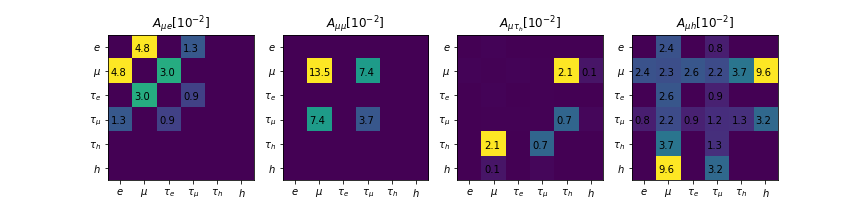
\includegraphics[width=0.8\textwidth,trim=3cm 0 3cm 0, clip]{chapters/Analysis/sectionStatisticalAnalysis/figures/acc_mu1b.png} \\
        % 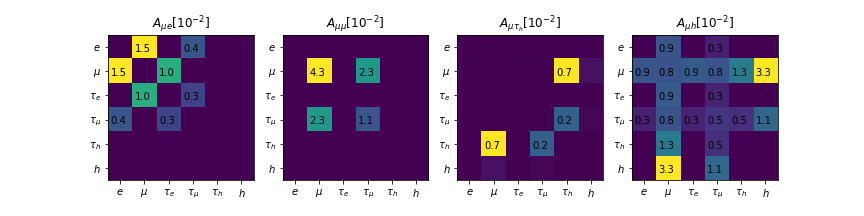
\includegraphics[width=0.7\textwidth]{chapters/Analysis/sectionStatisticalAnalysis/figures/acc_mu2b.png}
        % 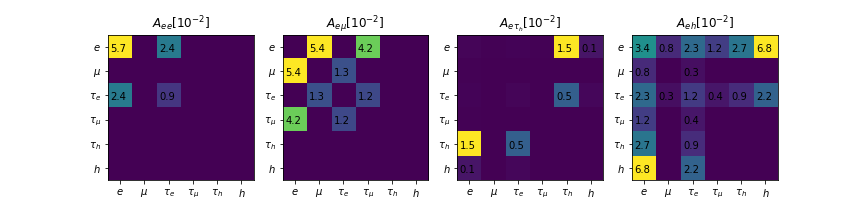
\includegraphics[width=0.7\textwidth]{chapters/Analysis/sectionStatisticalAnalysis/figures/acc_e1b.png}
        % 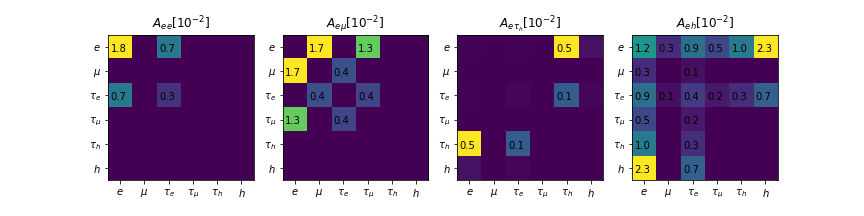
\includegraphics[width=0.7\textwidth]{chapters/Analysis/sectionStatisticalAnalysis/figures/acc_e2b.png}
       \footnotesize{ $\boldsymbol{E}$ matrix of \cme, \cmm, \cmt, \cmh channels with $n_j\geq2, n_b=1$.}
    \end{center}

    %\vspace{-0.08in}


    \footnotetext[1]{\tiny W+jets accounted for just using the vector $\beta$ and the corresponding vector of efficiencies.}
\end{frame}







\subsection{counting analysis}

% -------------
% new frame
% -------------
\begin{frame}{Counting analysis}
    % \begin{figure}
    %     \centering
    %     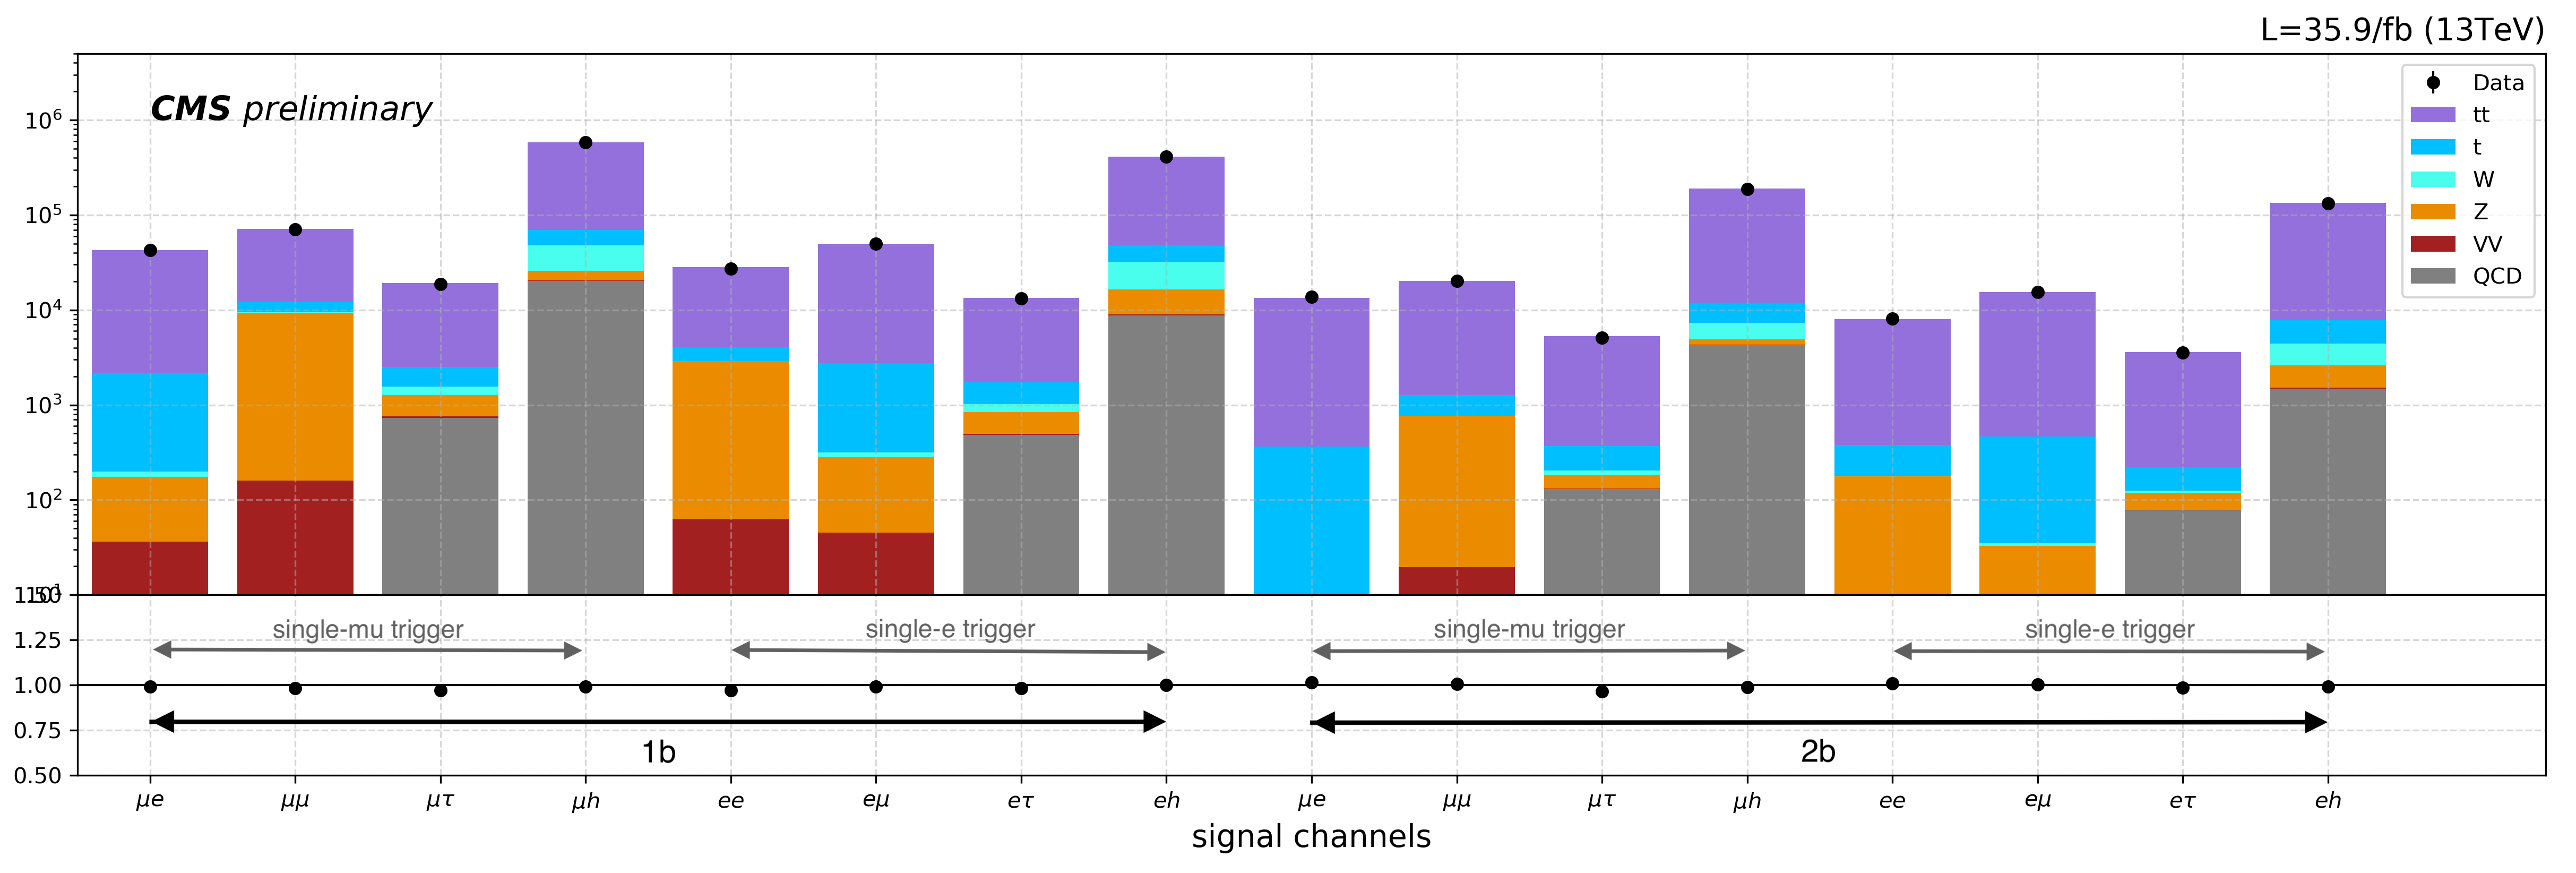
\includegraphics[width=0.9\textwidth]{chapters/Analysis/sectionStatisticalAnalysis/figures/counting.png}
    % \end{figure}

    \smaller
    For each of the trigger and $n_b$ regions, construct ratios \textcolor{NUpurple}{$\{X_{e},X_{\mu},X_{\tau}\}$} from data with background subtracted $n = N_{\rm data} - \sum N_{\rm bg}$,
    % Please add the following required packages to your document preamble:

    \begin{table}[]
        \centering
        \setlength{\tabcolsep}{2.5 em}
        \renewcommand{\arraystretch}{3}
        \resizebox{0.9\textwidth}{!}{
        \begin{tabular}{c|c|c|c|c}
        \rowcolor{NUpurple} 
                                & \multicolumn{2}{c|}{\textcolor{white}{Single-$\mu$ Trigger}}  & \multicolumn{2}{c}{\textcolor{white}{Single-$e$ Trigger}}    \\
        \rowcolor{NUpurple10} 
                                & $n_b = 1$                    & $n_b \geq 2$                   & $n_b = 1$                          & $n_b \geq 2$     \\ \hline 
        channels                & \multicolumn{2}{c|}{$\mu e$, $\mu \mu$, $\mu \tau_h$, $\mu h$} & \multicolumn{2}{c}{$e e$, $e \mu$, $e \tau_h$, $e h$}\\ \hline 
        \multirow{3}{*}{ratios, $t\in \{ \mu, e\}$} 
                                & \multicolumn{4}{c}{$\frac{n^{\ctre}  }{n^{\ctre} + n^{\ctrm} + n^{t\PGt} + n^{\ctrh}} = \textcolor{RedOrange}{X_\Pe   = \frac{ \Eij^{\ctre}\Bij }{  \Eij^{\ctre}\Bij+ \Eij^{\ctrm}\Bij+ \Eij^{t\PGt}\Bij+ \Eij^{\ctrh}\Bij}}$}\\
                                & \multicolumn{4}{c}{$\frac{n^{\ctrm}  }{n^{\ctre} + n^{\ctrm} + n^{t\PGt} + n^{\ctrh}} = \textcolor{Blue}{X_\PGm  = \frac{ \Eij^{\ctrm}\Bij }{  \Eij^{\ctre}\Bij+ \Eij^{\ctrm}\Bij+ \Eij^{t\PGt}\Bij+ \Eij^{\ctrh}\Bij}}$} \\
                                & \multicolumn{4}{c}{$\frac{n^{t\PGt}  }{n^{\ctre} + n^{\ctrm} + n^{t\PGt} + n^{\ctrh}} = \textcolor{OliveGreen}{X_\PGt  = \frac{ \Eij^{t\PGt}\Bij }{  \Eij^{\ctre}\Bij+ \Eij^{\ctrm}\Bij+ \Eij^{t\PGt}\Bij+ \Eij^{\ctrh}\Bij}}$} 
        \end{tabular}
        }
    \end{table}
    
   
\end{frame}



% -------------
% new frame
% -------------
\begin{frame}{}%Frame Title}
\smaller

    One gets a system of three quadratic equations with three unknowns $\{\bwe,\bwm,\bwt\}$,

    \begin{equation*}
    \tiny
	\begin{split}
        \textcolor{RedOrange}{F_\Pe(\bwe,\bwm,\bwt)} = c_{\Pe1} \bwe^2 + c_{\Pe2} \bwm^2 + c_{\Pe3} \bwt^2 + c_{\Pe4} \bwe\bwm + c_{\Pe5} \bwe\bwt + c_{\Pe6} \bwm\bwt + c_{\Pe7} \bwe + c_{\Pe8} \bwm + c_{\Pe9} \bwt + c_{\Pe0} &= 0 ,\\
        \textcolor{Blue}{F_\PGm(\bwe,\bwm,\bwt)} = c_{\PGm 1} \bwe^2 + c_{\PGm 2} \bwm^2 + c_{\PGm 3} \bwt^2 + c_{\PGm 4} \bwe\bwm + c_{\PGm 5} \bwe\bwt + c_{\PGm 6} \bwm\bwt + c_{\PGm 7} \bwe + c_{\PGm 8} \bwm + c_{\PGm 9} \bwt + c_{\PGm 0} &= 0, \\
        \textcolor{OliveGreen}{F_\PGt(\bwe,\bwm,\bwt)} = c_{_\PGt1} \bwe^2 + c_{\PGt2} \bwm^2 + c_{\PGt3} \bwt^2 + c_{\PGt4} \bwe\bwm + c_{\PGt5} \bwe\bwt + c_{\PGt6} \bwm\bwt + c_{\PGt7} \bwe + c_{\PGt8} \bwm + c_{\PGt9} \bwt + c_{\PGt0} &= 0 , \\
    \end{split}
    \end{equation*}
    
    where the coefficients $\{c_{ek},c_{\mu k},c_{\tau k} \}$ with $k\in\{ 0,1,2,\dots 9\}$ are fully determined by efficiencies $E$ and data ratios $\{X_e,X_\mu,X_\tau\}$.


	\begin{columns}[c] % align columns

	\column{.45\textwidth}
		\begin{figure}
			\centering
			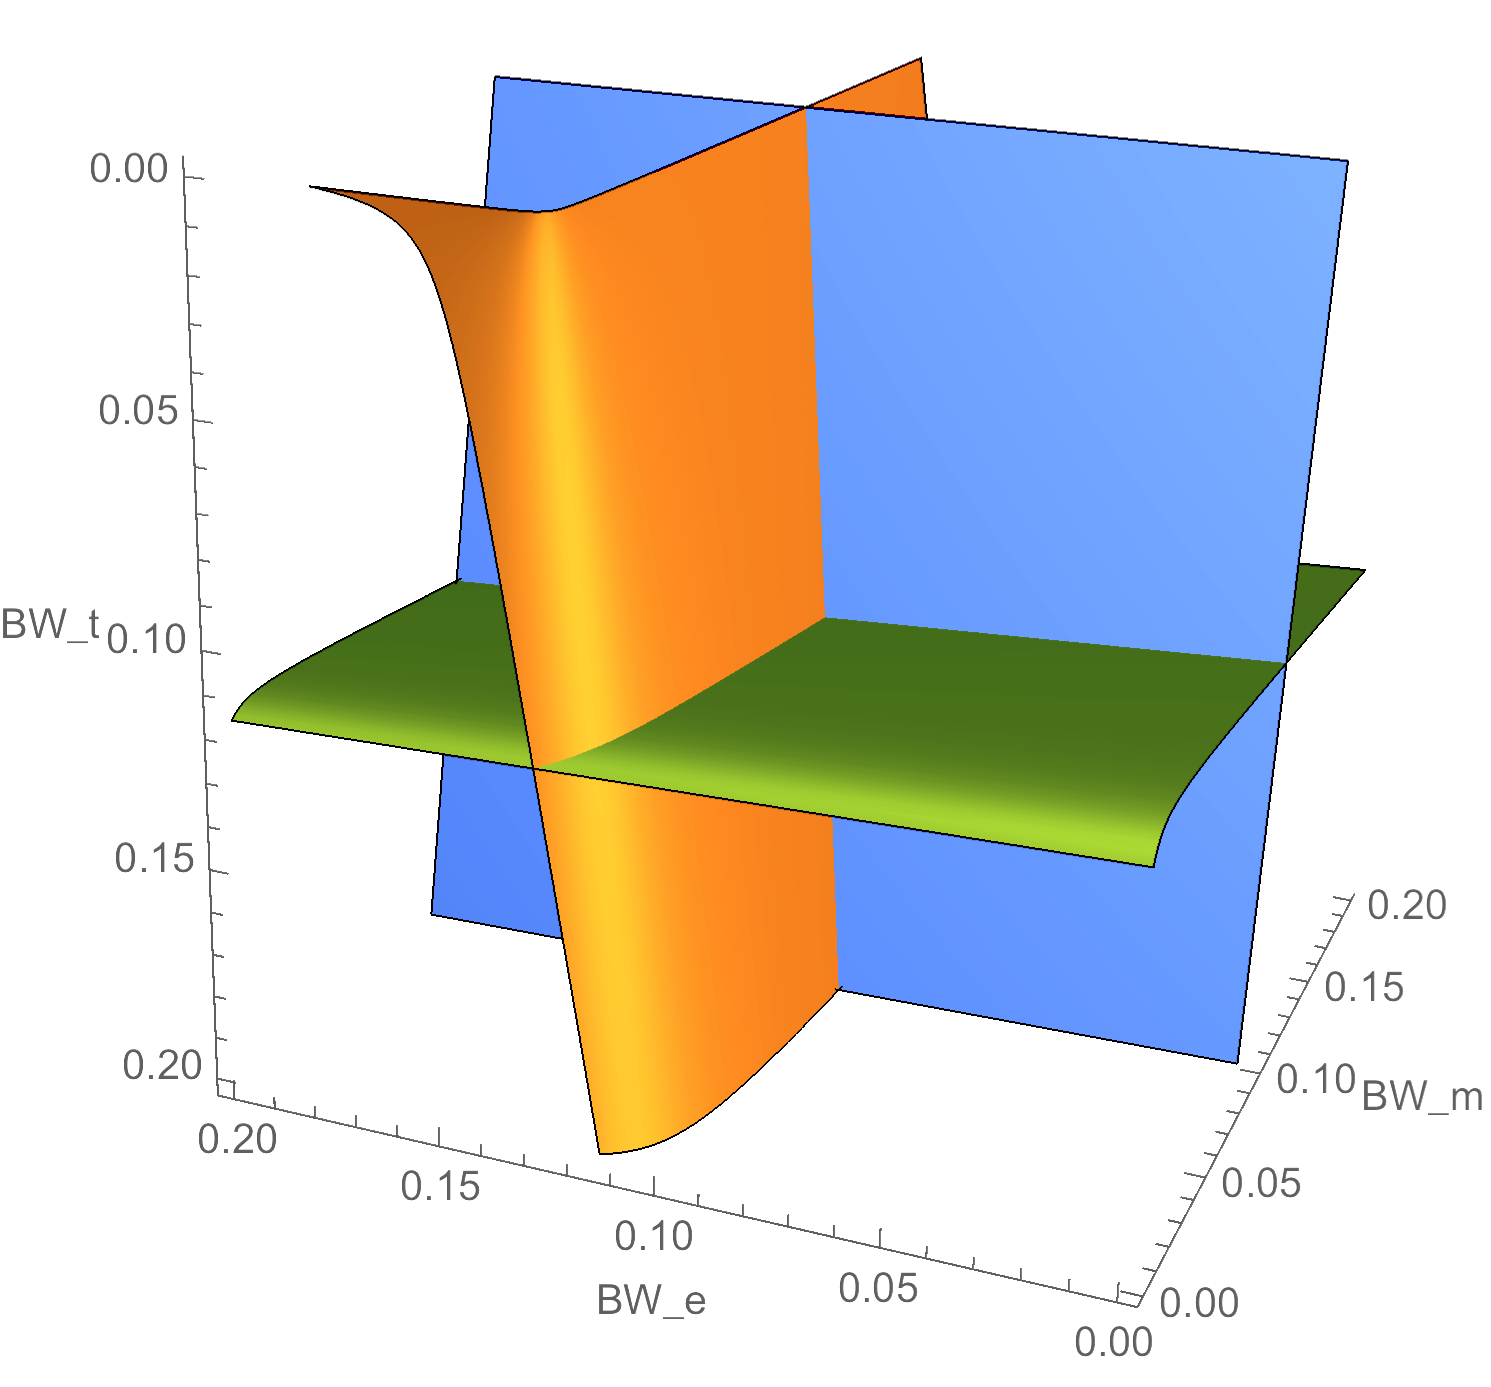
\includegraphics[width=0.9\textwidth]{chapters/Analysis/sectionStatisticalAnalysis/figures/visual.png}
		\end{figure}


	\column{.55\textwidth}
    \begin{itemize}
        \item In the $\{\beta_{e},\beta_{\mu},\beta_{\tau}\}$ space, three quadratic equations are three hyperbolic planes, intersection of which is the solution:
		\begin{equation*} 
            \small
            \begin{bmatrix} \bwe \\ \bwm \\ \bwt \end{bmatrix} = \text{Sol} 
                \begin{bmatrix}
                \textcolor{RedOrange}{F_\Pe (\bwe,\bwm,\bwt) = 0} \\
                \textcolor{Blue}{F_\PGm  (\bwe,\bwm,\bwt) = 0} \\
                \textcolor{OliveGreen}{F_\PGt (\bwe,\bwm,\bwt) = 0}
                \end{bmatrix}
		\end{equation*}
        \item The results from different trigger and $n_b$ categories are analytically combined by $\chi^2$ considering the uncorrelated statistical errors and correlated systematic error for any given systematic source.  
        \end{itemize}

	\end{columns}

\end{frame}





\subsection{shape analysis}

\begin{frame}{Shape analysis}
\smaller 
    \begin{columns}
        \column{0.6\textwidth}
        \begin{block}{\smaller discriminating $W\rightarrow e/\mu$ vs. $W\rightarrow\tau\rightarrow e/\mu$}
            \begin{itemize}
                \item Features are selected to best isolate
                    $W\rightarrow\tau$ decays 
                \begin{itemize}
                \smaller
                    \item \alert{$W\rightarrow\tau\rightarrow e/\mu$ tend to have lower \pt}
                \end{itemize}
                \item More sophisticated discrimination techniques considered, e.g.
                    neural networks, but...
                \begin{itemize}
                \smaller
                    \item lepton $\pt$ is by far still strongest source of discrimination
                    \item additional observables complicates treatment of systematic uncertainties
                \end{itemize}
                \item Trailing muon impact parameter considered (as for ATLAS), but requires extra calibration.
                \item Histograms binning are generated using the Bayesian Block algorithm \tiny{(B. Pollack, S. Bhattacharya, M. Schmitt, arXiv:1708.00810)}. 
            \end{itemize}

        \end{block}


        \column{0.4\textwidth}
        \begin{center}
            % \vspace{-0.1in} 
            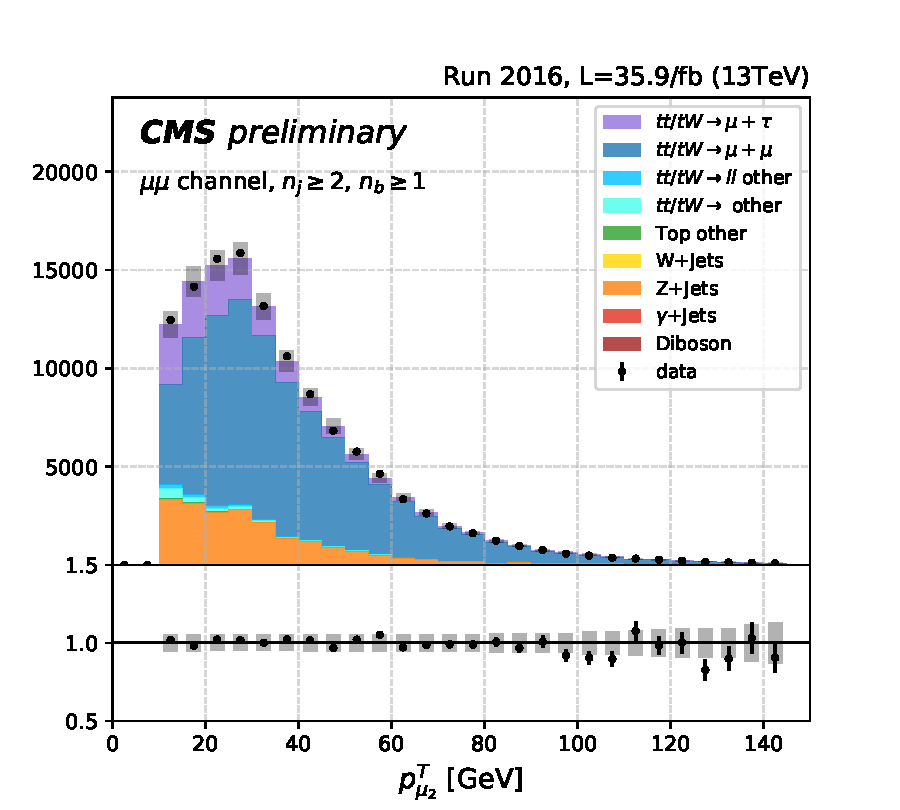
\includegraphics[width=0.9\textwidth]{chapters/Analysis/sectionPlots/figures/kinematics_pickles/mumu/12b/mumu_2b_lepton2_pt.pdf}
            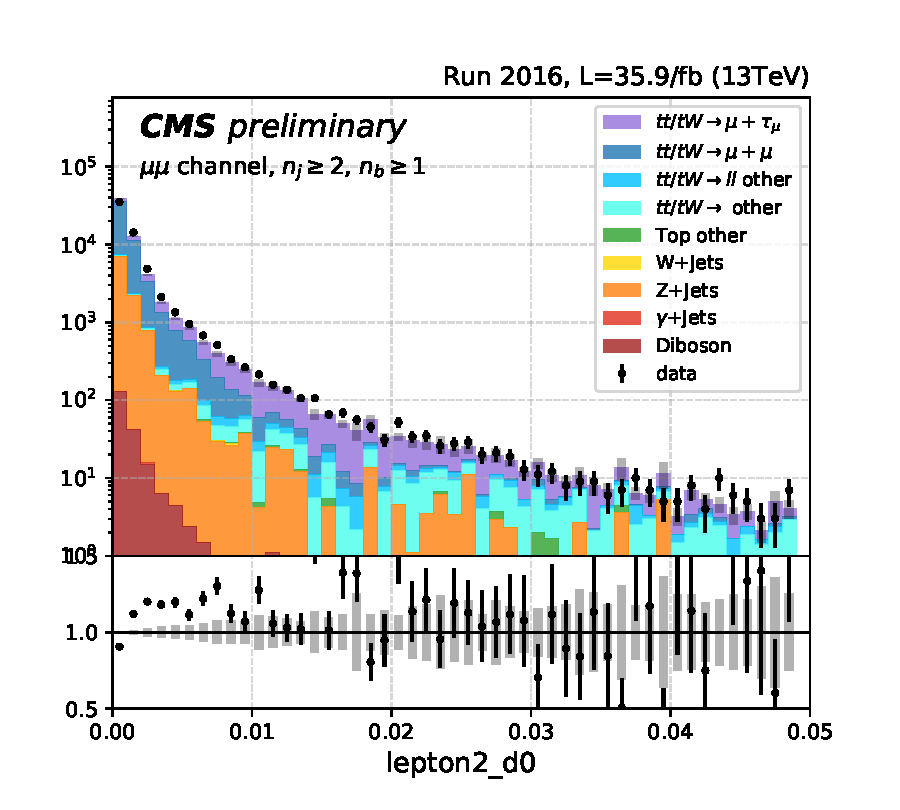
\includegraphics[width=0.9\textwidth]{chapters/Analysis/sectionSelection/figures/sob/mumu_lepton2_d0_logscale.pdf}
        \end{center}

    \end{columns}

\end{frame}


\begin{frame}{}
\smaller 

    \begin{block}{\smaller binned maximum likelihood estimation}
        In this case, the W branching fractions, $\mathbf{B}$, are treated as free parameters, and the values that minimize the NLL assuming Poisson probabilities are determined,

        \begin{equation*}
            \mathsf{NLL}(\boldsymbol{B}, \boldsymbol{\theta}|\mathbf{y}) = \sum_{\mathsf{i\in category}} 
            \sum_{\mathsf{j \in bins}} -y_{ij}\ln(f_{ij}(\boldsymbol{B}, \boldsymbol{\theta})) + f_{ij}(\boldsymbol{B}, \boldsymbol{\theta}) + \sum_{k\in n.p.}\pi_\theta (\theta)
        \end{equation*}

        where $y_{ij}$ is the data yield in category $i$ and bin $j$, and $f_{ij}$ is the prediction
        parameterized by the branching fractions, $\mathbf{B}$ and nuisance parameters,
        $\boldsymbol{\theta}$. The constraint on the n.p. are denoted by $\pi_{\theta}(\theta)$. The
        data model is written, 

        \begin{equation*}
            f_{ij}(\boldsymbol{B}, \boldsymbol{\theta}) = \sum_{s\in sig} s_{ij,s}(\boldsymbol{B}, \boldsymbol{\theta}) + \sum_{b\in bg} b_{ij,b}(\boldsymbol{\theta}). 
        \end{equation*}

    \end{block}

    \begin{itemize}
        \smaller
        \item 30 categories based on jet and b tag multiplicities;
        \item total of 74 template components, w/ only $\sim 10$ are relevant to any specific category;
        \item $\sim 100$ non-MC stat nuisance parameters;
        \item $\sim 400$ bins in total;
        \item template morphing and MC stat. variation implemented according to arXiv:1103.0354;
        \item minimization using \textcolor{blue}{\texttt{scipy.optimize.minimize}}
    \end{itemize}
    
\end{frame}



\begin{frame}{} %$ee$ and $\mu\mu$: trailing lepton $\pt$}
Post-fit distributions

    \begin{columns}
        \column{0.5\textwidth}
        \begin{tcolorbox}[colframe=NUpurple]{ \cee and \cmm: trailing lepton $\pt$}
            \begin{center}
                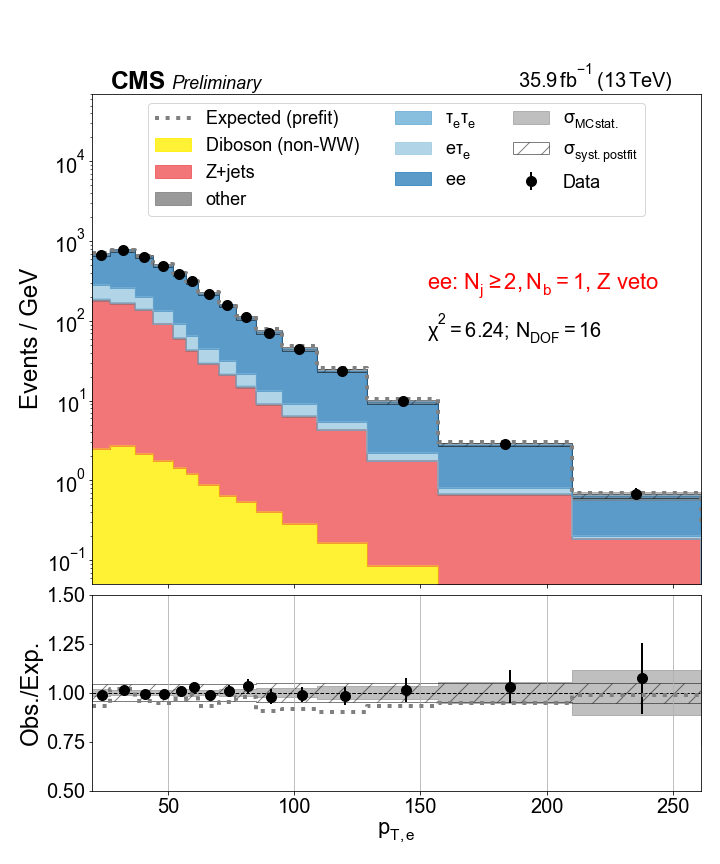
\includegraphics[width=0.48\textwidth]{chapters/Analysis/sectionStatisticalAnalysis/figures/fit/ee_cat_gt2_eq1_b}
                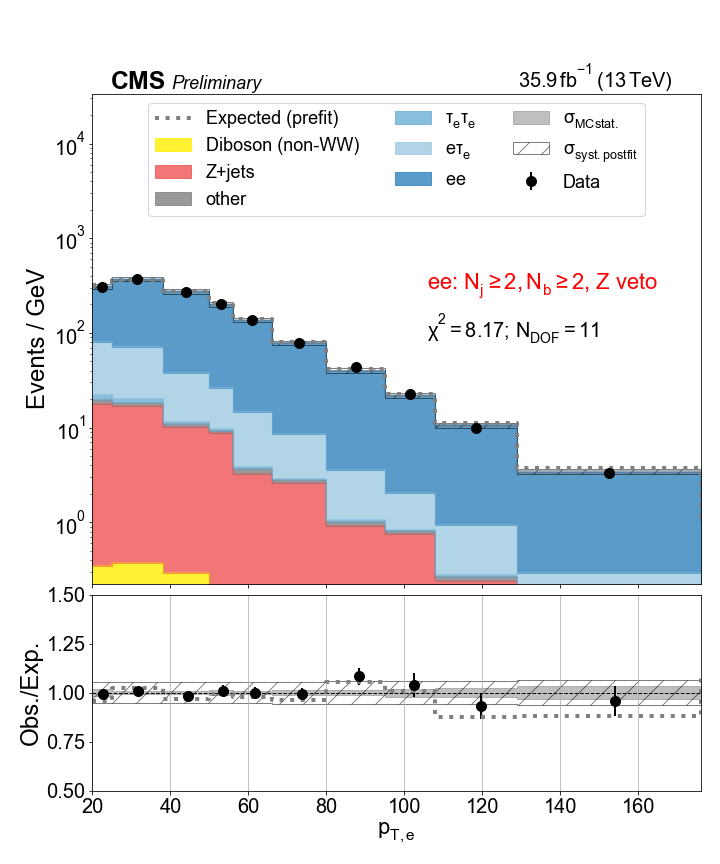
\includegraphics[width=0.48\textwidth]{chapters/Analysis/sectionStatisticalAnalysis/figures/fit/ee_cat_gt2_gt2_b}

                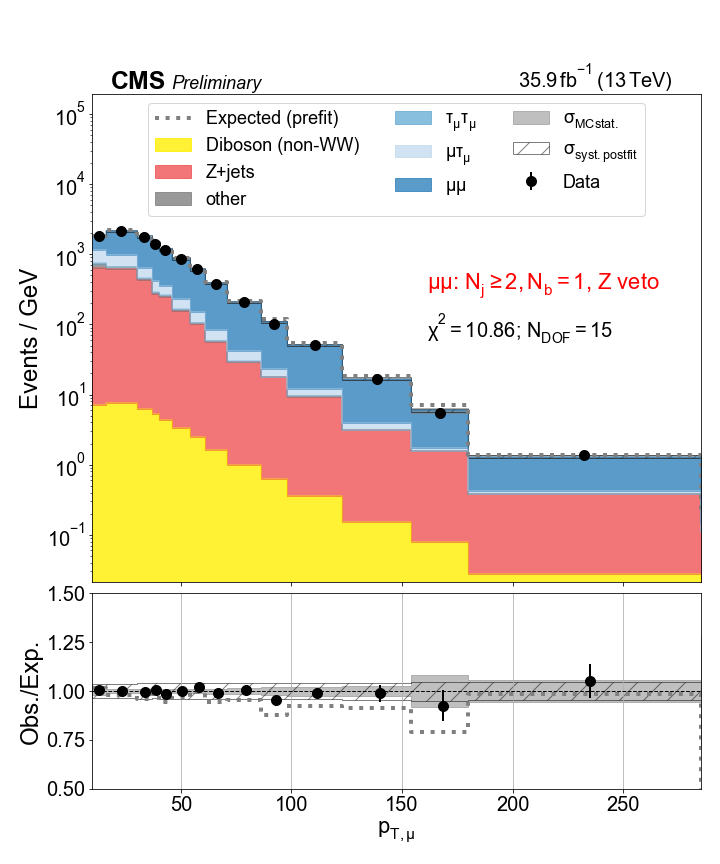
\includegraphics[width=0.48\textwidth]{chapters/Analysis/sectionStatisticalAnalysis/figures/fit/mumu_cat_gt2_eq1_b}
                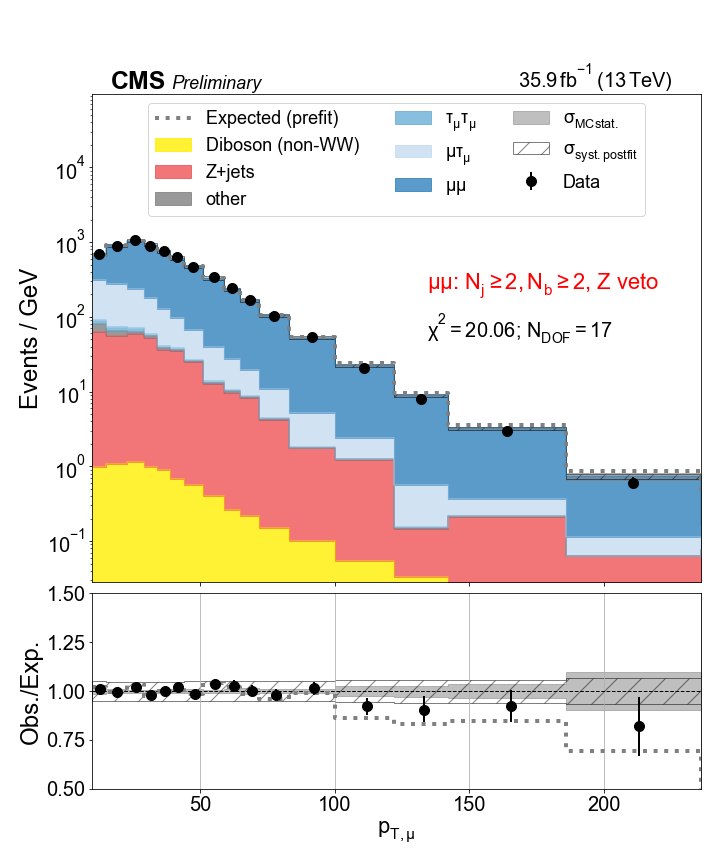
\includegraphics[width=0.48\textwidth]{chapters/Analysis/sectionStatisticalAnalysis/figures/fit/mumu_cat_gt2_gt2_b}
            \end{center}
        \end{tcolorbox}{}

        \column{0.5\textwidth}
        \begin{tcolorbox}[colframe=NUpurple]{ \ceh and \cmh: lepton $\pt$}
            \begin{center}
                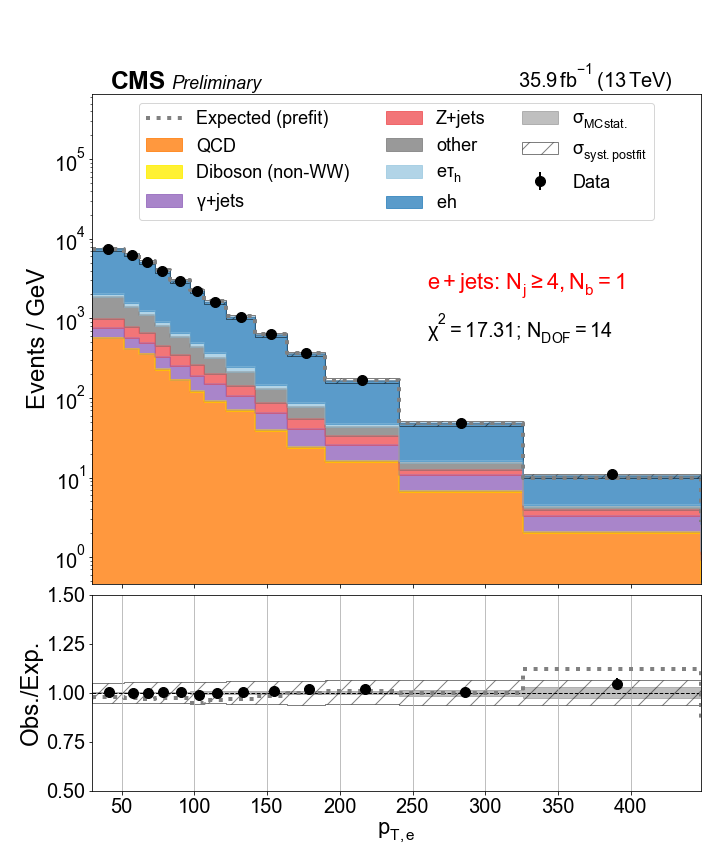
\includegraphics[width=0.48\textwidth]{chapters/Analysis/sectionStatisticalAnalysis/figures/fit/ejet_cat_gt4_eq1}
                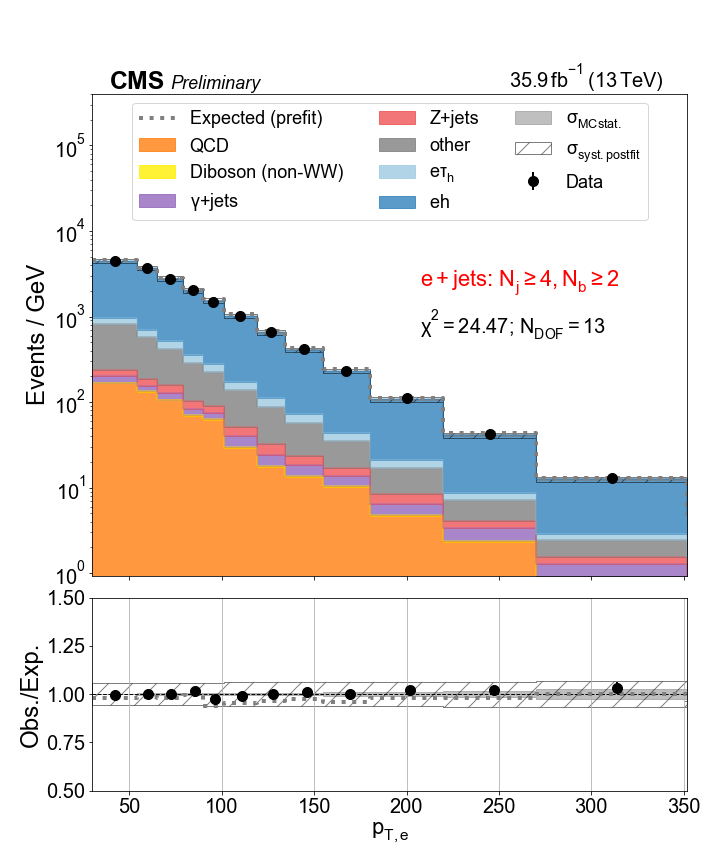
\includegraphics[width=0.48\textwidth]{chapters/Analysis/sectionStatisticalAnalysis/figures/fit/ejet_cat_gt4_gt2}

                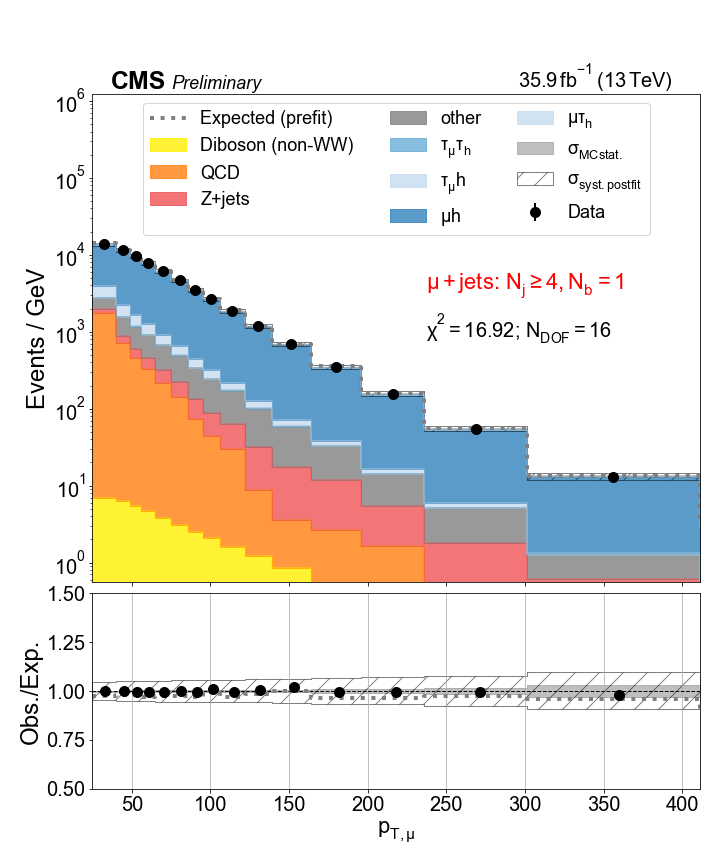
\includegraphics[width=0.48\textwidth]{chapters/Analysis/sectionStatisticalAnalysis/figures/fit/mujet_cat_gt4_eq1}
                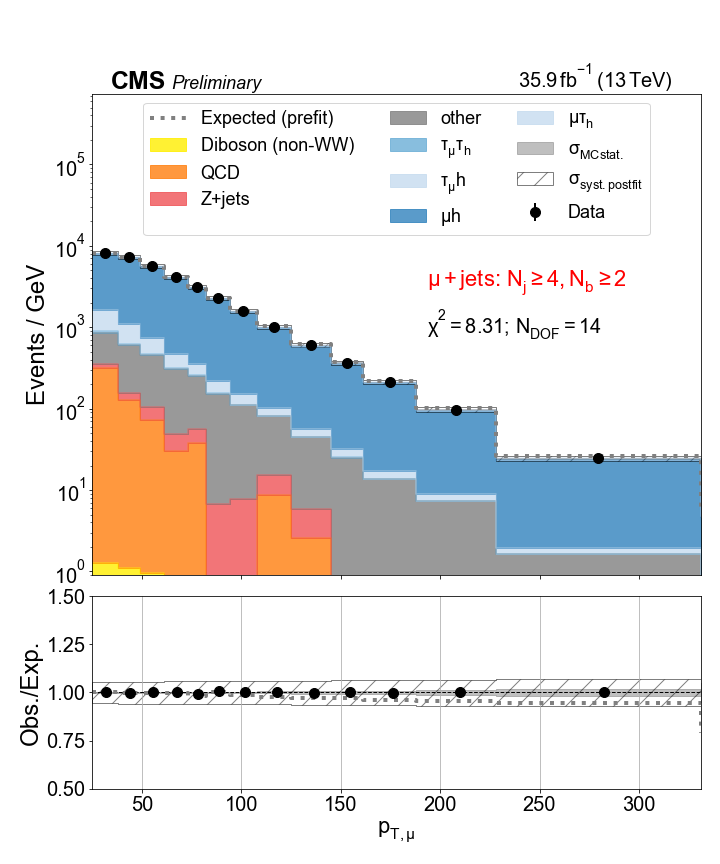
\includegraphics[width=0.48\textwidth]{chapters/Analysis/sectionStatisticalAnalysis/figures/fit/mujet_cat_gt4_gt2}
            \end{center}
        \end{tcolorbox}
    \end{columns}

\end{frame}

\begin{frame}{}
Post-fit distributions
    \begin{tcolorbox}[colframe=NUpurple]{ \cem: trailing lepton $\pt$}
        \begin{center}
            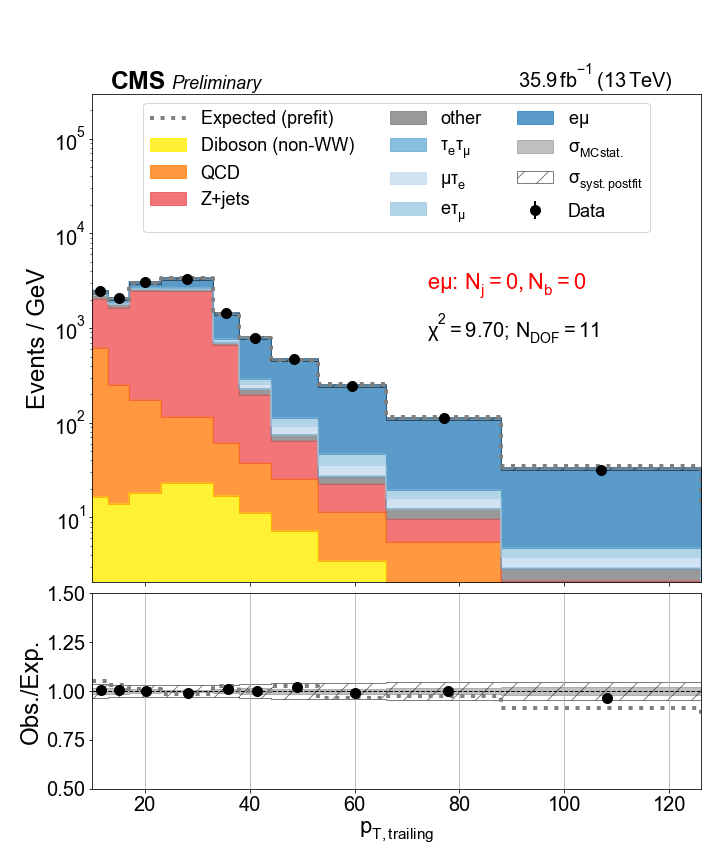
\includegraphics[width=0.25\textwidth]{chapters/Analysis/sectionStatisticalAnalysis/figures/fit/emu_cat_eq0_eq0_a}
            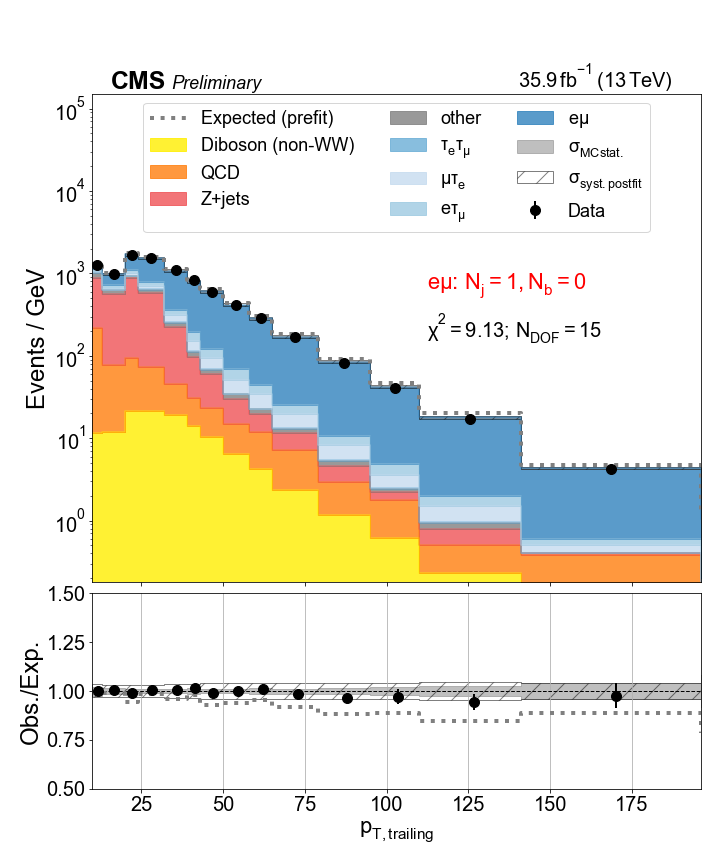
\includegraphics[width=0.25\textwidth]{chapters/Analysis/sectionStatisticalAnalysis/figures/fit/emu_cat_eq1_eq0_a}
            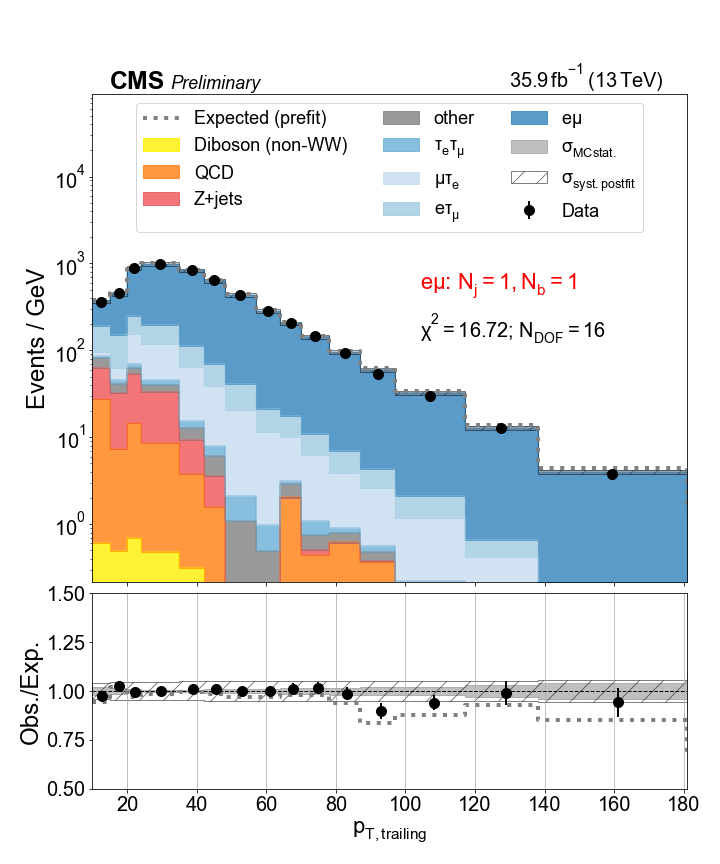
\includegraphics[width=0.25\textwidth]{chapters/Analysis/sectionStatisticalAnalysis/figures/fit/emu_cat_eq1_eq1_a}

            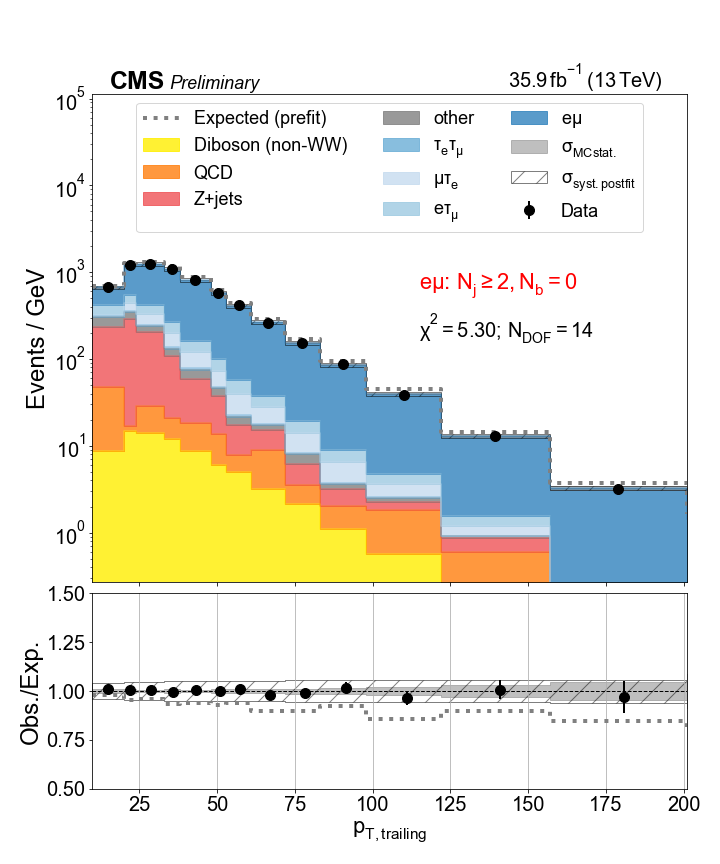
\includegraphics[width=0.25\textwidth]{chapters/Analysis/sectionStatisticalAnalysis/figures/fit/emu_cat_gt2_eq0}
            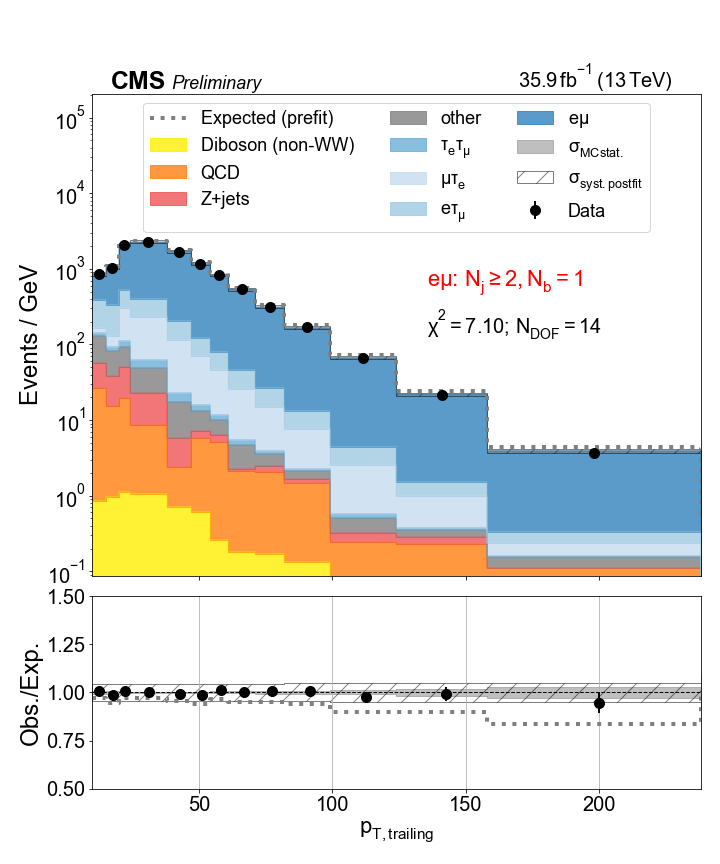
\includegraphics[width=0.25\textwidth]{chapters/Analysis/sectionStatisticalAnalysis/figures/fit/emu_cat_gt2_eq1_a}
            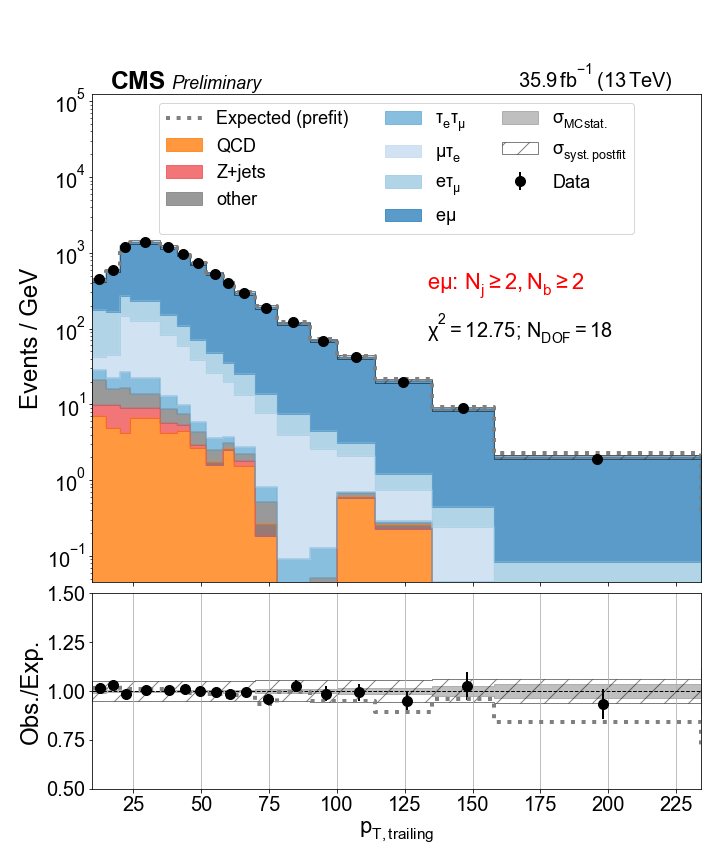
\includegraphics[width=0.25\textwidth]{chapters/Analysis/sectionStatisticalAnalysis/figures/fit/emu_cat_gt2_gt2_a}
        \end{center}
    \end{tcolorbox}

\end{frame}

\begin{frame}{}
Post-fit distributions
    \begin{tcolorbox}[colframe=NUpurple]{ \cet: tau $\pt$}
        \begin{center}
            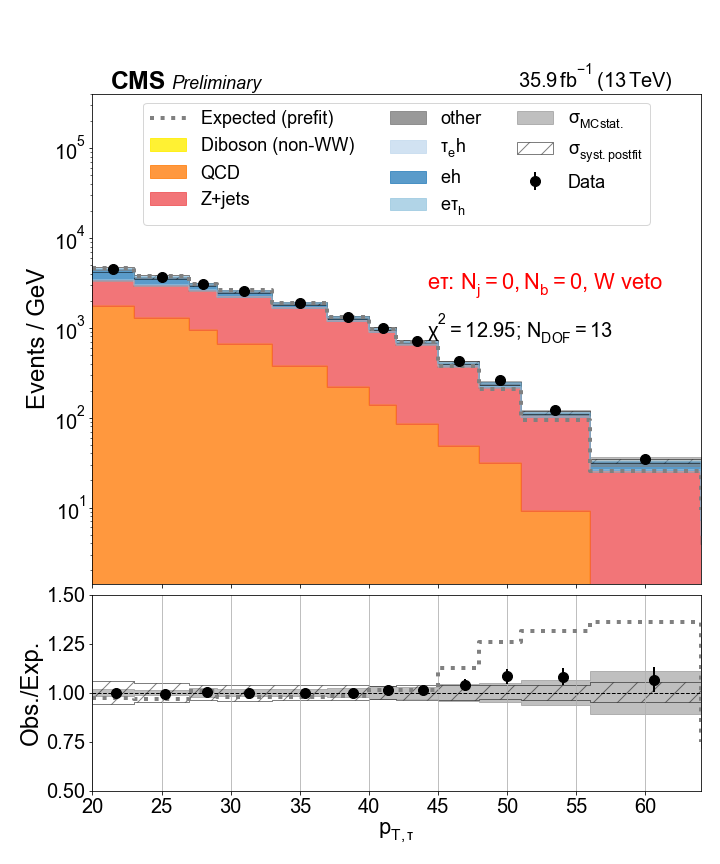
\includegraphics[width=0.24\textwidth]{chapters/Analysis/sectionStatisticalAnalysis/figures/fit/etau_cat_eq0_eq0}
            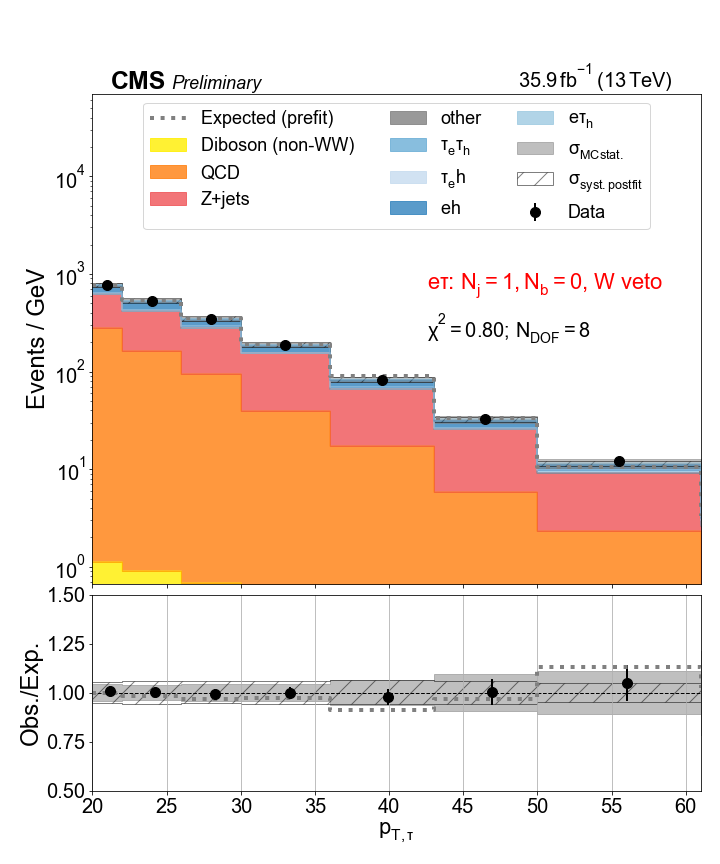
\includegraphics[width=0.24\textwidth]{chapters/Analysis/sectionStatisticalAnalysis/figures/fit/etau_cat_eq1_eq0}
            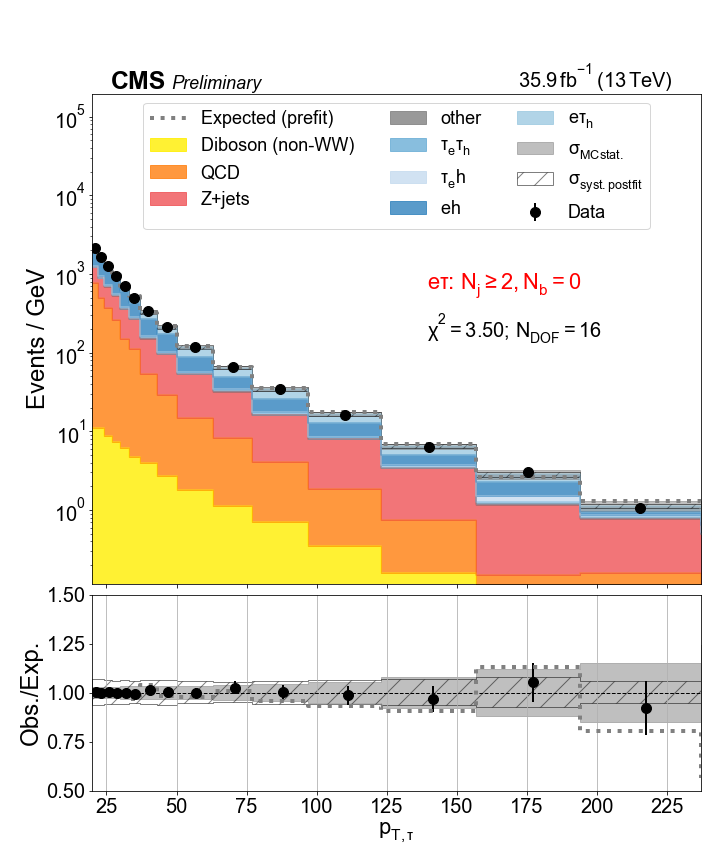
\includegraphics[width=0.24\textwidth]{chapters/Analysis/sectionStatisticalAnalysis/figures/fit/etau_cat_gt2_eq0}
            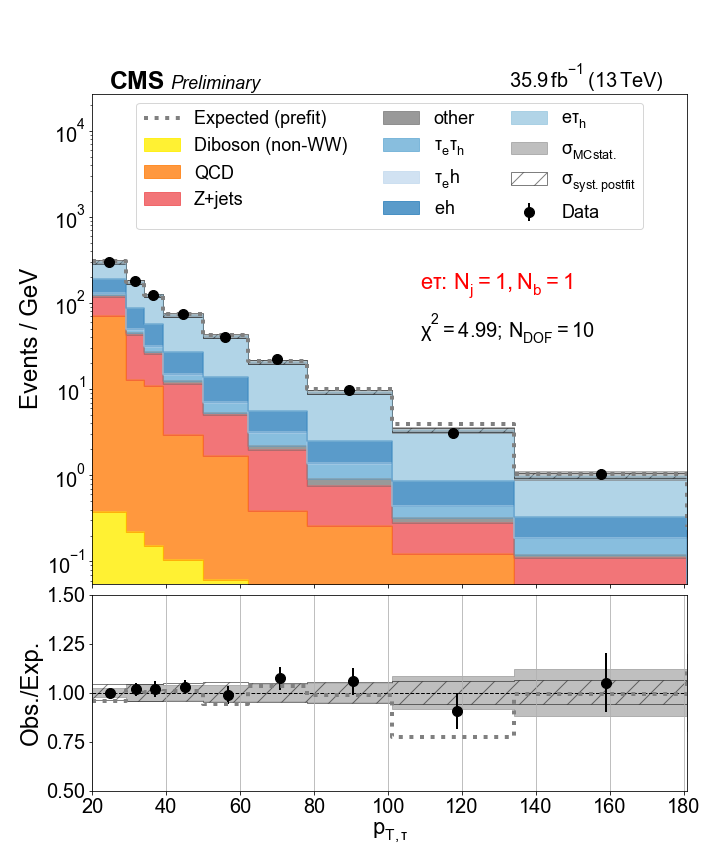
\includegraphics[width=0.24\textwidth]{chapters/Analysis/sectionStatisticalAnalysis/figures/fit/etau_cat_eq1_eq1}

            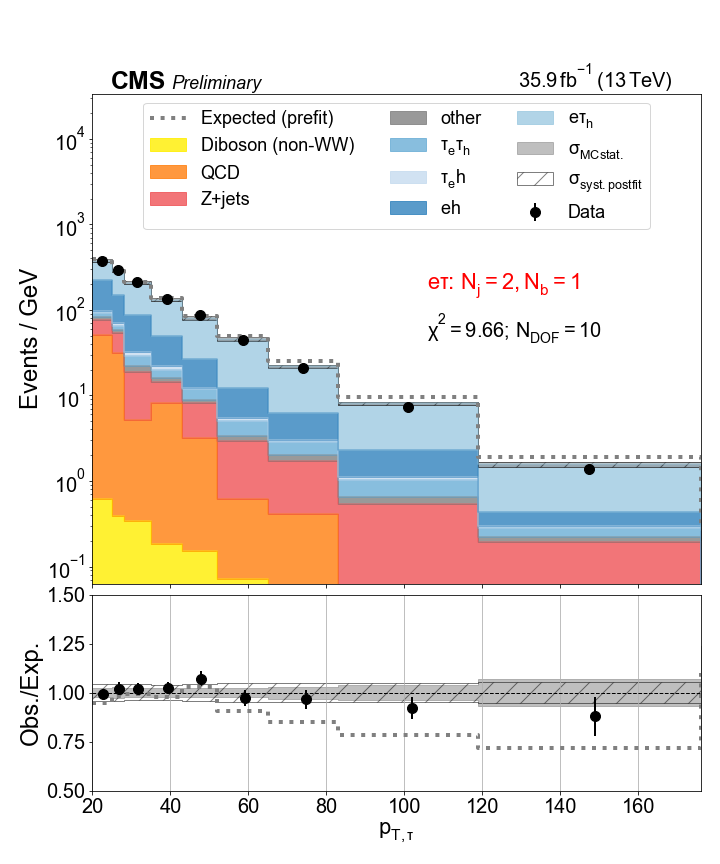
\includegraphics[width=0.24\textwidth]{chapters/Analysis/sectionStatisticalAnalysis/figures/fit/etau_cat_eq2_eq1}
            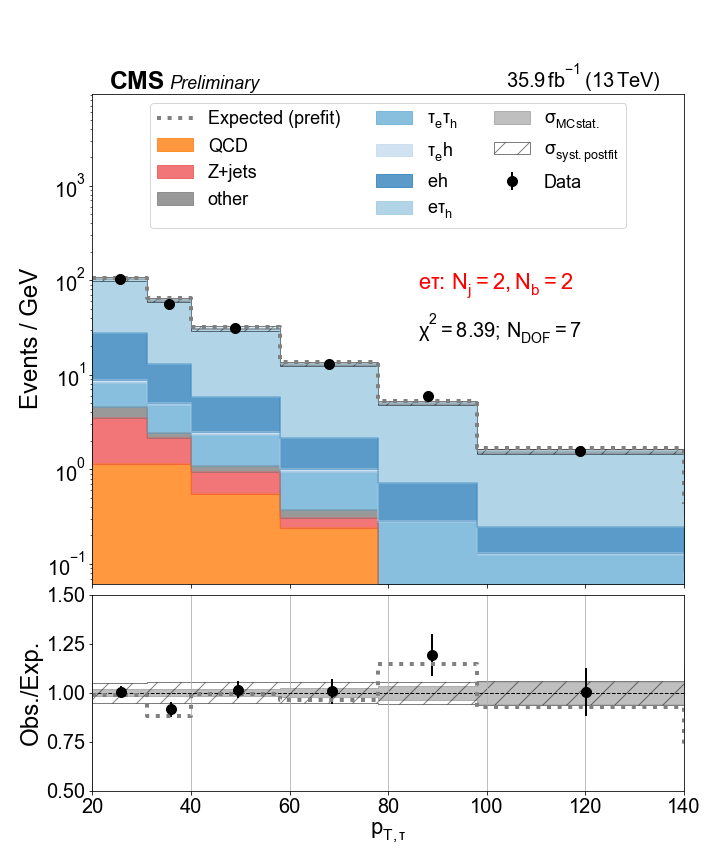
\includegraphics[width=0.24\textwidth]{chapters/Analysis/sectionStatisticalAnalysis/figures/fit/etau_cat_eq2_eq2}
            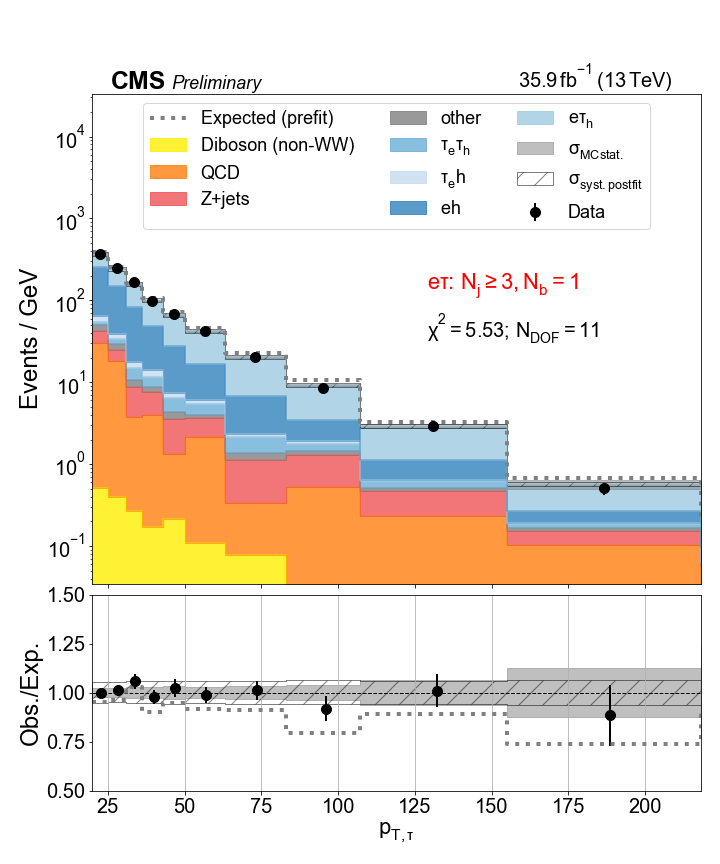
\includegraphics[width=0.24\textwidth]{chapters/Analysis/sectionStatisticalAnalysis/figures/fit/etau_cat_gt3_eq1}
            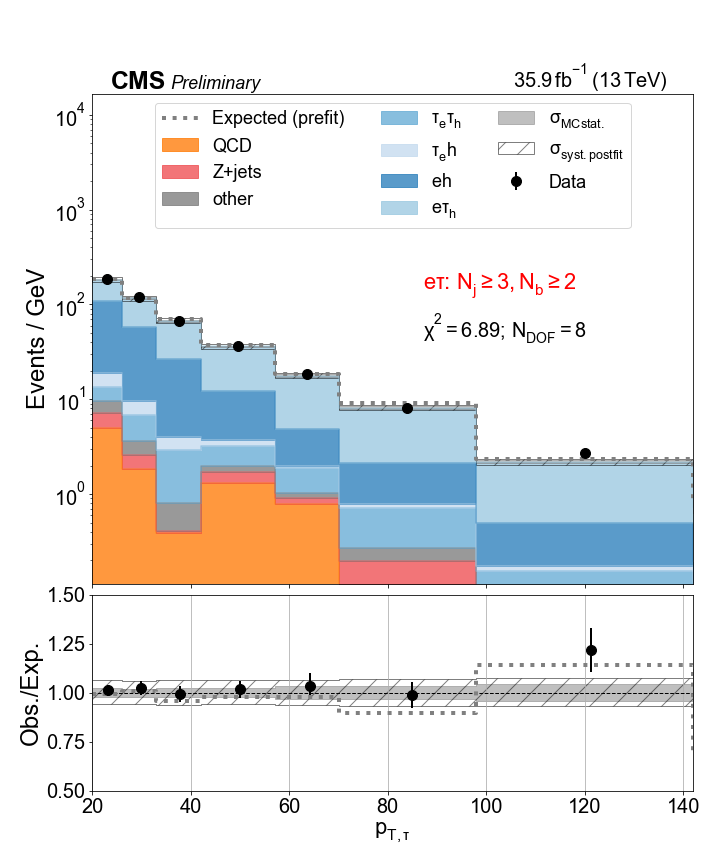
\includegraphics[width=0.24\textwidth]{chapters/Analysis/sectionStatisticalAnalysis/figures/fit/etau_cat_gt3_gt2}
        \end{center}
    \end{tcolorbox}
\end{frame}

\begin{frame}{}
Post-fit distributions
    \begin{tcolorbox}[colframe=NUpurple]{ \cmt: tau $\pt$}
        \begin{center}
            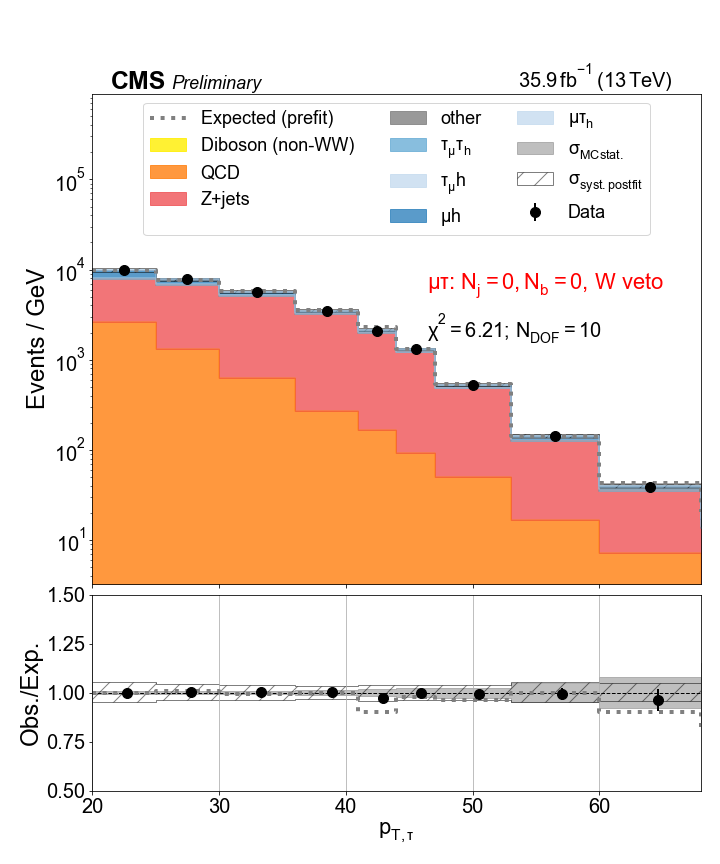
\includegraphics[width=0.24\textwidth]{chapters/Analysis/sectionStatisticalAnalysis/figures/fit/mutau_cat_eq0_eq0}
            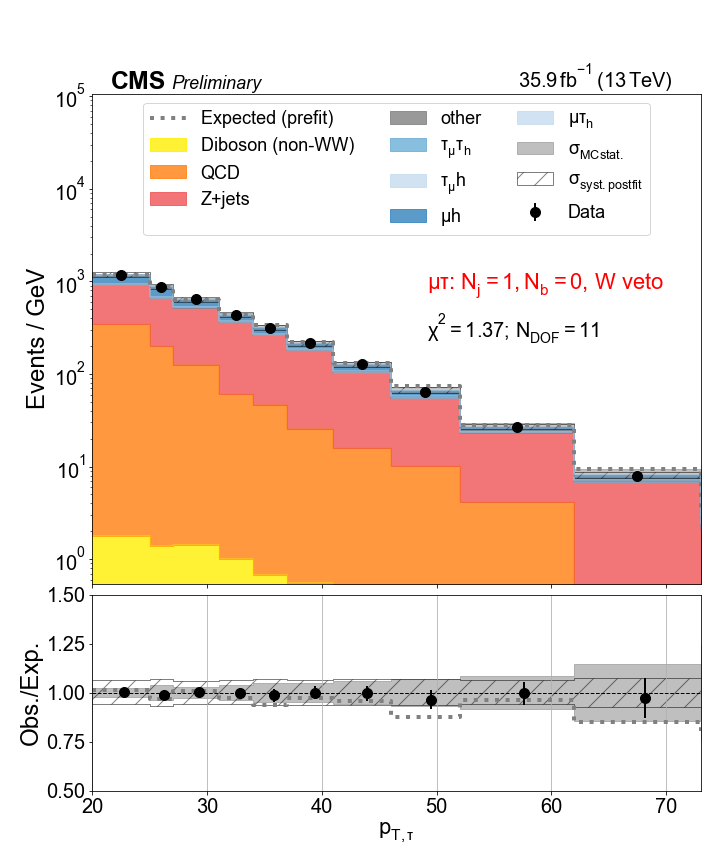
\includegraphics[width=0.24\textwidth]{chapters/Analysis/sectionStatisticalAnalysis/figures/fit/mutau_cat_eq1_eq0}
            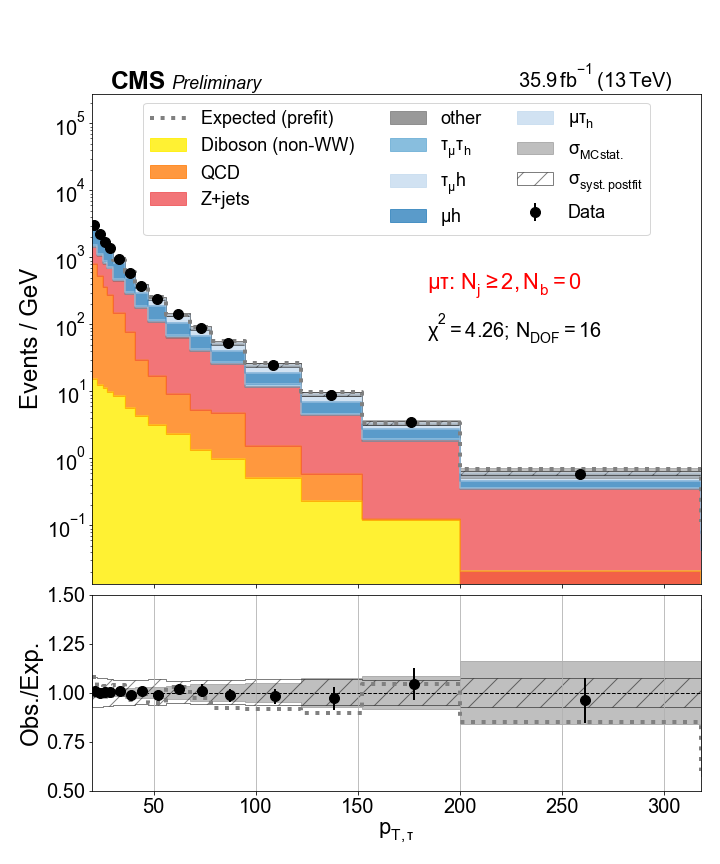
\includegraphics[width=0.24\textwidth]{chapters/Analysis/sectionStatisticalAnalysis/figures/fit/mutau_cat_gt2_eq0}
            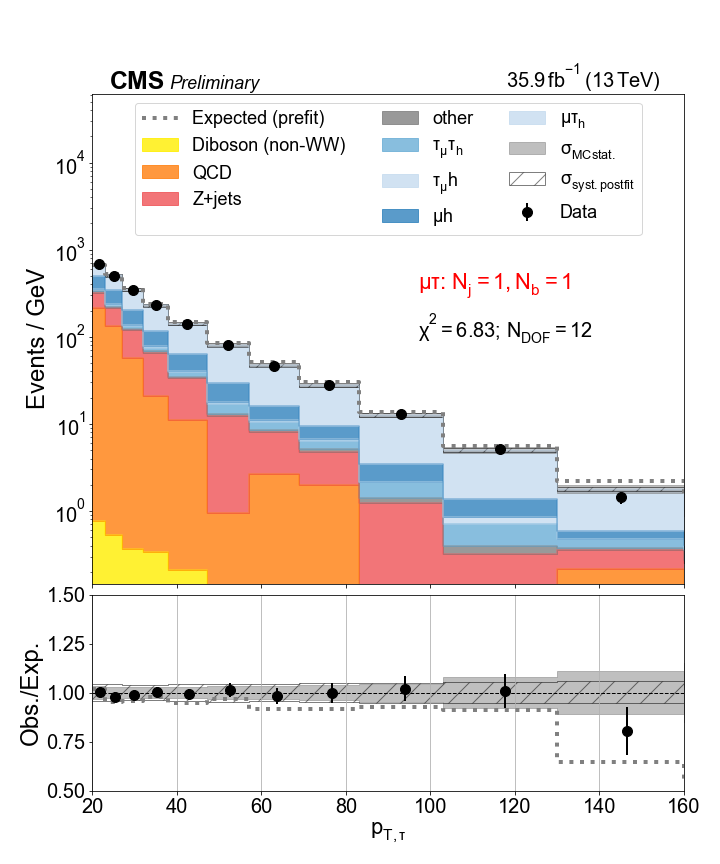
\includegraphics[width=0.24\textwidth]{chapters/Analysis/sectionStatisticalAnalysis/figures/fit/mutau_cat_eq1_eq1}

            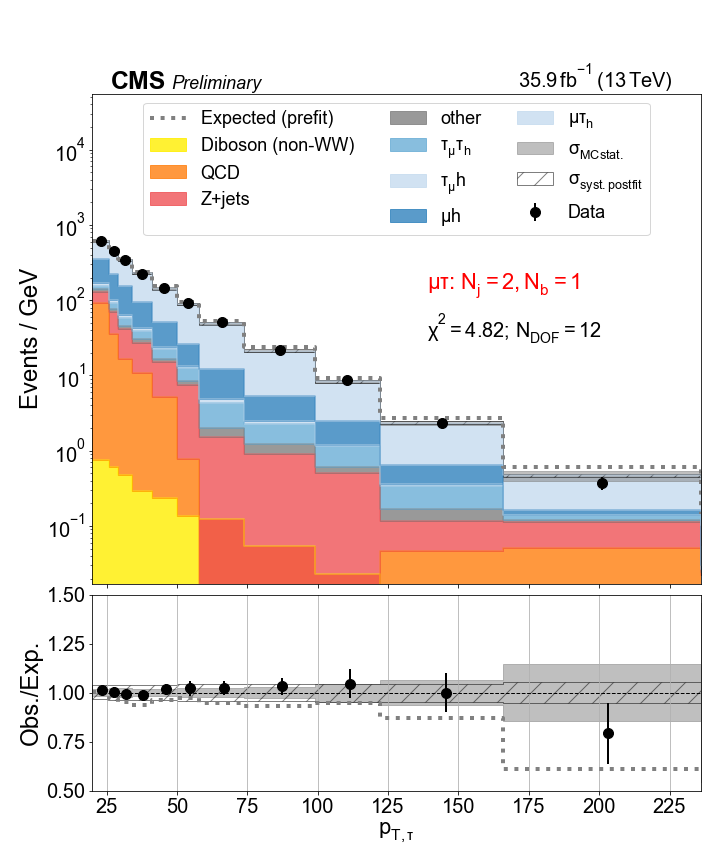
\includegraphics[width=0.24\textwidth]{chapters/Analysis/sectionStatisticalAnalysis/figures/fit/mutau_cat_eq2_eq1}
            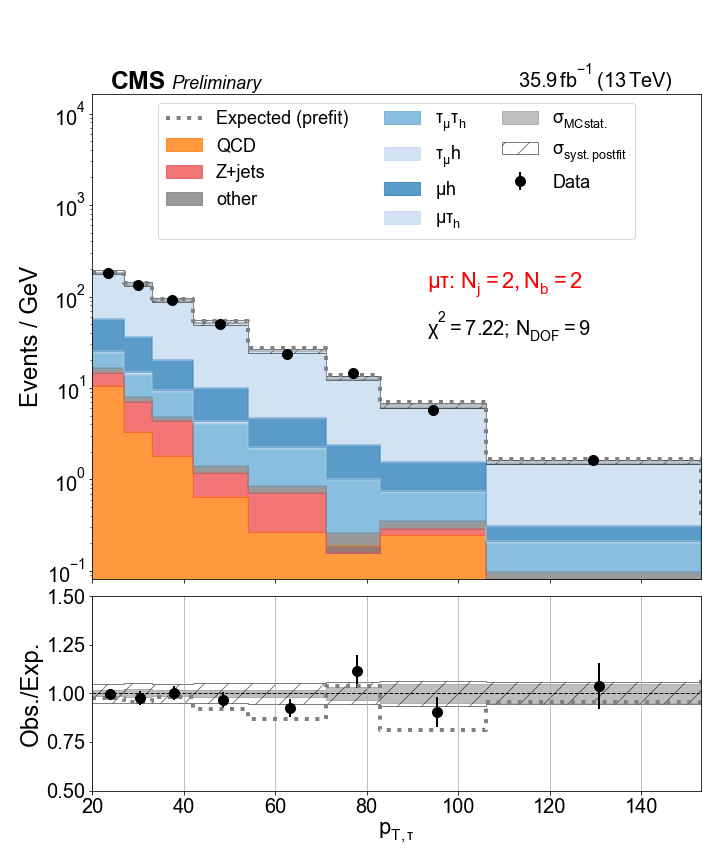
\includegraphics[width=0.24\textwidth]{chapters/Analysis/sectionStatisticalAnalysis/figures/fit/mutau_cat_eq2_eq2}
            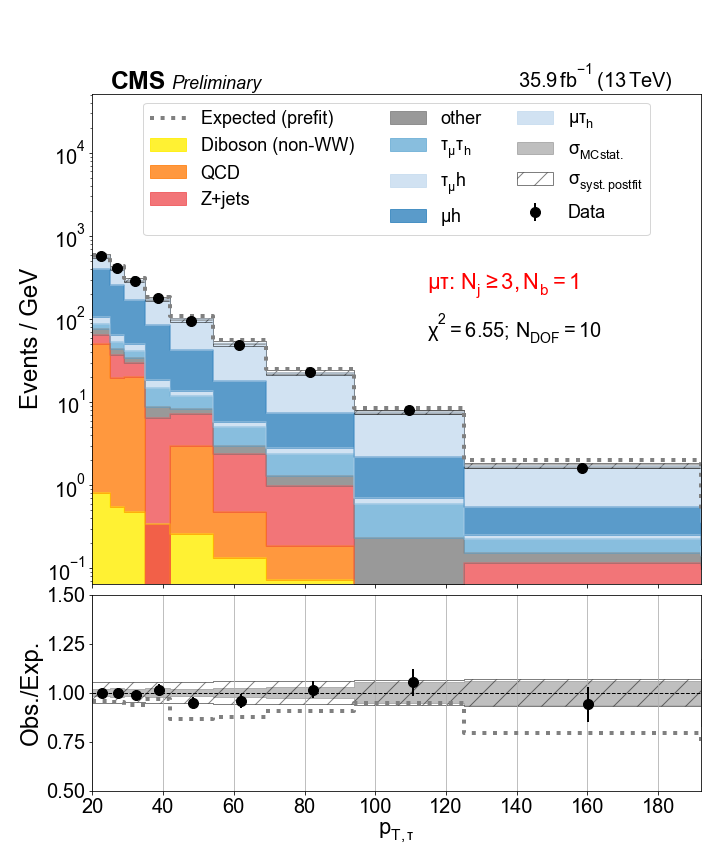
\includegraphics[width=0.24\textwidth]{chapters/Analysis/sectionStatisticalAnalysis/figures/fit/mutau_cat_gt3_eq1}
            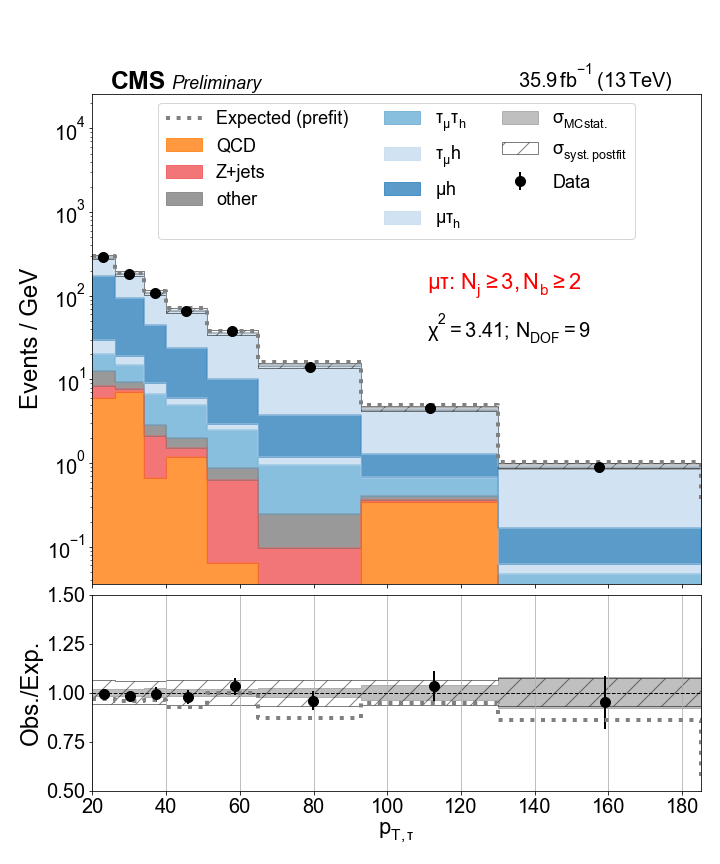
\includegraphics[width=0.24\textwidth]{chapters/Analysis/sectionStatisticalAnalysis/figures/fit/mutau_cat_gt3_gt2}
        \end{center}
    \end{tcolorbox}

\end{frame}
